\chapter{Introduction}
\label{chap:intro}

This thesis work takes place in the context of the ShieldBot project, which aims to revolutionize the construction, renovation, and maintenance sectors by investigating and validating a new generation of robotic systems tailored to the industry's unique challenges \cite{shieldbot_project}. The ShieldBot project focuses on three complementary robotic solutions:

\begin{itemize}
    \item InnerShieldBot is designed for internal construction works to enhance the thermal performance of walls and ceilings.
    \item InspectionShieldBot is dedicated to identify structural or insulation needs, and ensure long-term building integrity.
    \item FaçadeShieldBot is designed to operate on building façades and install thermal shielding in order to improve insulation and reduce energy consumption.
\end{itemize}

\begin{figure}[h]
    \centering
    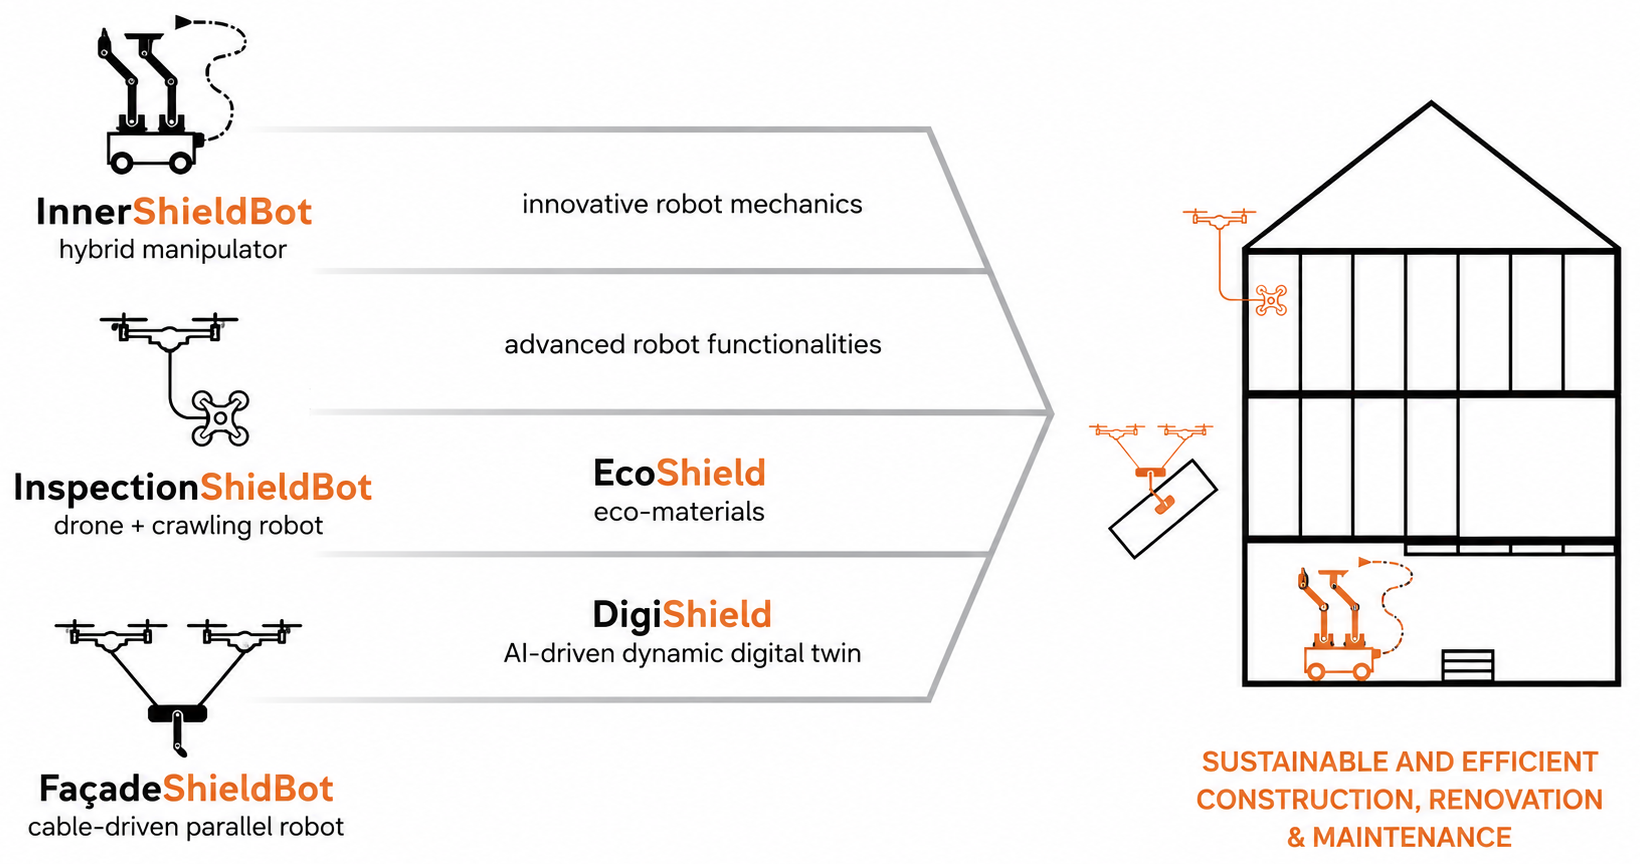
\includegraphics[width=\linewidth]{images/ShieldBot_About_TheProject_Graph_01.png}
    \caption{Robotic solutions developed by the ShieldBot project \cite{shieldbot_project}}
    \label{fig:shieldbotGraph}
\end{figure}

\noindent This thesis focuses on the challenges associated with using the Façade\-Shield\-Bot robot. Here, the system must generate sufficient force to manipulate a robotic arm mounted on
the payload while maintaining a stable pose, as the application requires transporting and accurately positioning a payload near a vertical surface. However, the scope of this work is strictly centered on the aerial platform itself and its ability to maintain a controlled pose without relying on permanent building infrastructure.

% Existing cable-driven robots provide high precision but rely on fixed environmental anchors
Previous robotic developments have demonstrated the potential of cable-based systems for construction applications. For example, the TitanBot project investigates cable-driven parallel robotic (CDPR) systems capable of transporting loads over large areas and reducing the physical effort required from construction workers \cite{cnrs_titanbot_2025}. Such systems benefit from the mechanical simplicity and large workspace offered by cable-based actuation. What is even more interesting is that this configuration allows their actuators to be positioned at a distance from the load to be moved, making them particularly suitable for applications involving heavy loads. However, conventional configurations generally rely on fixed or ground-based cable attachment points, which can limit their flexibility when operating over complex or changing environments.


\begin{figure}[h]
    \centering
    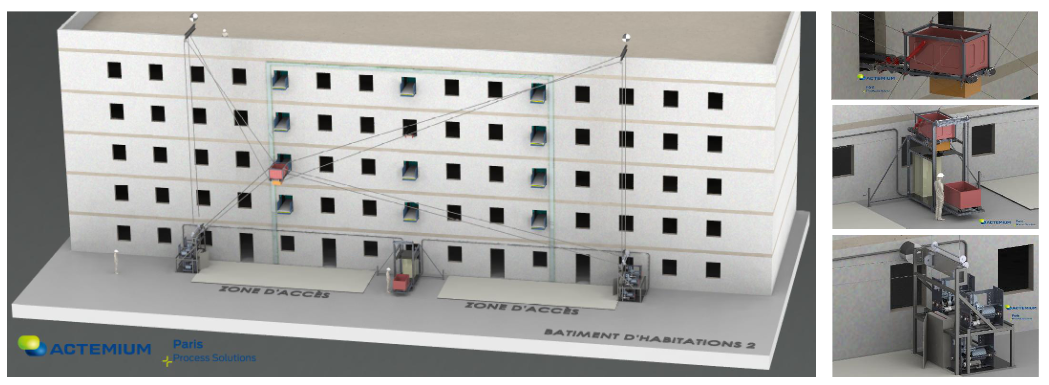
\includegraphics[width=\linewidth]{images/titanbot.png}
    \caption{Solution proposed by TitanBot project \cite{cnrs_titanbot_2025}}
    \label{fig:titanbot}
\end{figure}

% Aerial Cable-Towed Systems increase flexibility but suffer from reduced positioning accuracy.
Aerial robotic systems are a promising approach to access tight and difficult-to-reach areas while reducing the need for traditional scaffolding. Additionally, the use of cables introduces distance between the UAVs and the building, removing direct contact between the two (Figure \ref{fig:acts_constrain}). This is advantageous from a safety and operational perspective, as it reduces the risk of unintended collisions and the impact of the airflow generated by the rotors, allowing the system to safely come into contact with vertical surface \cite{erskine_control_2019}.

\begin{figure}[h]
    \centering
    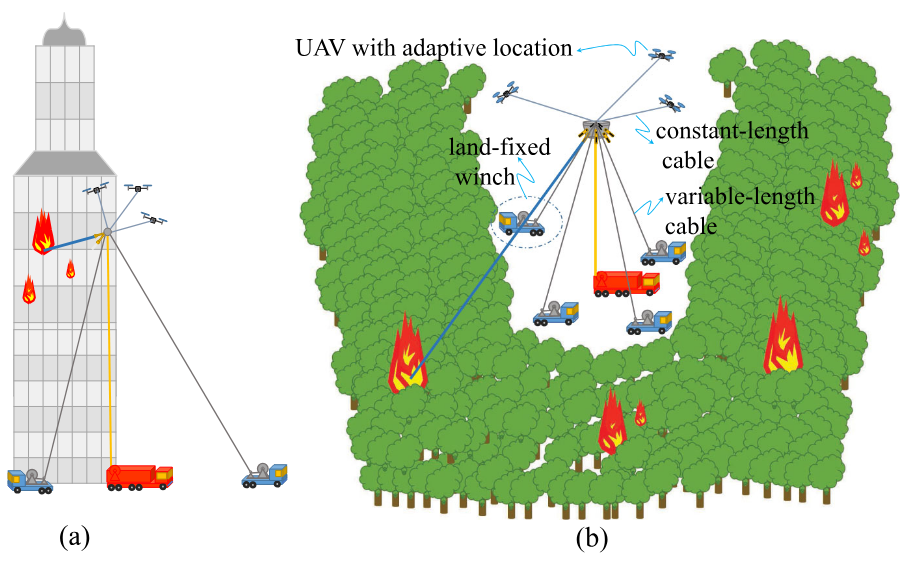
\includegraphics[width=0.7\linewidth]{Images/acts_use.png}
    \caption{Using ACTRs with land-fixed winches for firefighting applications on (a) high-rise buildings and (b) vast areas such as forests \cite{jamshidifar_static_2020}}
    \label{fig:acts_constrain}
\end{figure}

Nonetheless, the position and orientation of the UAVs directly influence the forces and moments that can be generated through the cables. As a result, accurate positioning of the payload can become difficult, particularly when the system is required to perform precise manipulation close to a façade. These limits are especially critical in applications where the payload needs to be precisely positioned and then manipulated against a vertical surface.

% Hybrid aerial-ground systems attempt to combine the advantages of both approaches.
The combination of aerial and ground-based actuation can improve the ability of the system to generate and control forces during interaction with the façade while retaining the flexibility of an aerial cable-towed system.
% However, the influence of cable routing, attachment locations and architecture selection on system performance has received limited attention.
The resulting system, however, is characterized by a large set of design parameters that need to be selected at the design stage and remain fixed during the operation. They strongly influence the workspace, wrench feasibility, controllability, robustness, and energy efficiency of the system. The main design degrees of freedom include:

\begin{itemize}
    \item The number of aerial and ground vehicles (UAVs and UGVs), which determines the level of actuation redundancy and force distribution capability;
    \item The number of cables and their routing, which affect the achievable wrench set and the system's stability;
    \item The cable length actuation strategy, such as fixed-length or winch-actuated cables;
    \item The system architecture and graph rigidity, including centralized and decentralized control configurations.
\end{itemize}

As a result, architectural design cannot be isolated from control system development. A configuration that is mechanically feasible may nevertheless provide poor force distribution or positioning performance in the region of interest. Conversely, an appropriate choice of architecture and attachment locations can improve the controllability and robustness of the system without necessarily increasing its mechanical complexity.

% This thesis addresses this gap by...
The main objective of this thesis is to study the modelling, design, and control of a hybrid Aerial Cable-Towed System (ACTS) for payload manipulation. In particular, the thesis focuses on how the selection of suitable cable routing and attachment configurations to the payload influence the ability of the system to manipulate the payload itself and generate the required payload wrench. The proposed configurations are evaluated through simulation to assess their performance and identify the most suitable architecture for the considered application. 
The thesis is organized as follows.

Chapter \ref{chap:state_of_art} reviews the state of the art on cooperative cable-driven aerial systems, comparing Cable-Driven Parallel Robots (CDPRs), Aerial Cable-Towed Systems (ACTSs), and Flying Parallel Robots (FPRs), and discusses existing approaches to environmental interaction and to the control of cable-suspended UAV systems.

Chapter \ref{chap:design_modeling} develops the kinematostatic model of the ACTS and introduces the architecture design problem, including the relevant design variables, feasibility conditions (WCC, WFC, IFC), performance indices, and the proposed selection strategy for candidate cable routings.

Chapter \ref{chap:control} presents the control architecture, starting from simplified point-mass payload cases and extending progressively to the complete ACTS, including the payload-level wrench controller, the tension-distribution optimizer, and the UAV cascade control.

Chapter \ref{chap:simulation} describes the simulation environment and experimental setup, motivating the choice of MuJoCo over Gazebo, and details the software architecture used to generate, simulate, and evaluate candidate ACTS configurations.

Chapter \ref{chap:results} presents the simulation results, including the validation of the Stewart-platform baseline, the comparison of ground cable routings, the study of ground-anchor spacing, and the analysis of UAV attachment topologies.

Chapter \ref{chap:conclusions} summarizes the main findings of the thesis and outlines directions for future work.